\chapter{算法应用——Bin-Picking}
\label{chap:app}
本章主要介绍3D-MRAI算法的实际应用——Bin-Picking。首先介绍一下Bin-Picking相关背景,以及近些年的具体研究与发展;然后详细介绍基于3D-MRAI算法所开发的一套解决Bin-Picking问题的视觉系统,包括硬件的选型、开发环境、系统的框架设计以及算法的具体实现;最后介绍了针对所开发的Bin-Picking视觉系统,进行了随机抓取的实验,测试了系统抓取的成功率以及系统的抓取速度。

\section{Bin-Picking背景与现状}
使用机器人分拣散乱的工件的问题,在学术上我们称之为Bin-Picking,Bin-Picking并不是一个崭新的问题,学术上对这个问题的研究以及有了五十多年的历史。典型的Bin-Picking系统主要包括三部分:机器人、视觉检测模块和计算机控制模块。其中,视觉检测模块是整个Bin-Picking系统的核心部分,通过视觉检测模块对存放散乱工件的物料箱进行分析,获取目标工件的位姿,计算机控制模块根据视觉检测模块的检测结果规划机器人的运动路径,然后机器人执行完成工件的抓取。

传统的Bin-Picking中检测估计目标工件的算法大致可以分为两类:一类是基于特征匹配的算法,另一类是基于模板匹配的算法。基于特征匹配的算法,通过某些特征描述目标工件,如边角、空洞等特征,然后通过分析特征在空间中的旋转变换和平移变换来估计目标零件的位姿。这一类方法受工件纹理或者结构以及传感器的精度影响很大。另外一类基于模板匹配的方法的精度受限与模板的数量,要获得较高的精度就需要大量的模板,而大量的模板会造成算法运行时间过长。

工业上用于解决Bin-Picking问题的视觉系统也有许多,如图\ref{fig:bin-picking-sys}所示。日本的Fanuc公司推出了基于iRVision的Bin-Picking系统,该系统通过四个相机进行三维视觉重建,然后进行目标定位\cite{connolly2007new}。德国的ISRA Vision公司推出了3D Shape Scan系统,丹麦的Scape Technologies公司推出了Scape-Tech Discs系统,德国的Sick公司退出了PLB-500系统,诸如类似的Bin-Picking系统还有许多,这些Bin-Picking系统的价格大多二十万以上,并且抓取成功率和速度也往往难以满足客户需求,因此工业上还是缺少成熟的、价格便宜的、抓取成功率高、速度快的Bin-Picking解决方案。
\begin{figure}[ht]
  \centering
  \subfloat[Fanuc的iRVision系统]{\includegraphics[width=6cm]{fanuc}}
  \hskip1.5cm
  \subfloat[ISRA Vision的3D Shape Scan系统]{\includegraphics[width=6cm]{3dshape}}
  \vfill
  \subfloat[Scape Technologies的Scape-Tech Discs系统]{\includegraphics[width=6cm]{scapetech}}
  \hskip1.5cm
  \subfloat[Sick的PLB-500系统]{\includegraphics[width=6cm]{plb500}}
  \caption{工业上典型的Bin-Picking解决方案}
  \label{fig:bin-picking-sys}
\end{figure}

随着近几年一些高性价比的3D相机的出现,如微软的Kinect系列、Intel的RealSense系列,加上近几年深度学习的巨大发展,使得开发一种性价比高的、抓取成功率高的、速度快的Bin-Picking系统成为可能。但尽管深度学习在计算机视觉领域(Computer Vision)有了大量的研究,但在机器人感知(Robot Perception)领域的应用还比较少,因此本文将深度学习在计算机视觉领域内的成果通过一些改进引入到Robot Perception领域,再结合传统的全局点云匹配算法,提除了3D-MRAI算法,可以用于解决Bin-Picking相关问题。此外,本文基于Intel的RealSense SR300相机所提出的对偶RGB-D相机构建也为整个Bin-Picking系统提供了高性价比的相机解决方案。

\section{基于3D-MRAI的随机分拣系统}
\subsection{系统硬件设计}
本文所设计的基于3D-MRAI的随机分拣系统的硬件系统如图\ref{fig:hardware-sys}所示。
\begin{figure}[ht]
  \centering
  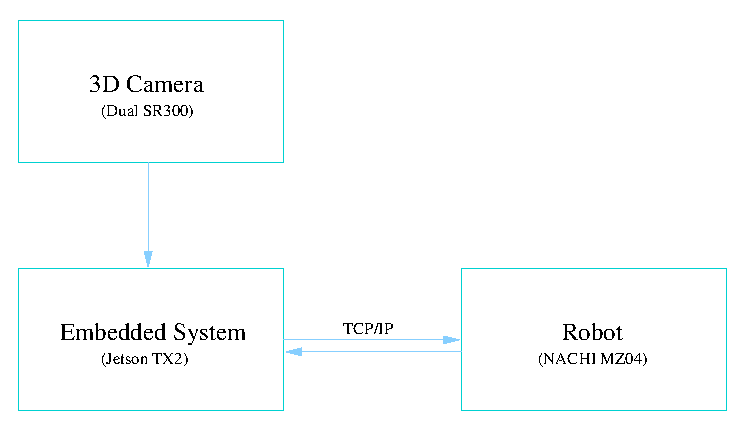
\includegraphics[width=14cm]{hardware-sys}
  \caption{基于3D-MRAI的随机分拣系统硬件框架}
  \label{fig:hardware-sys}
\end{figure}
从图\ref{fig:hardware-sys}可以看出,所设计的随机分拣系统的硬件系统由三个部分构成:相机模块、嵌入式计算模块以及机器人模块。对于相机模块,根据3D-MRAI算法的输入,需要相机能采集RGB-D图像,并且考虑整个系统的响应时间以及价格因此,希望相机模块的采集时间尽可能短,性价比尽可能高,因此选用了以结构光为原理的3D相机,并根据第~\ref{chap:rgbd}~章所设计的对偶RGB-D相机,用两个SR300相机构成了对偶RGB-D相机模块。

嵌入式计算模块选用了搭载了NVDIA公司的Jetson TX2模块的嵌入式计算机,如图\ref{fig:embeded-system},Jetson TX2如图\ref{fig:jetsontx2}所示。
\begin{figure}[ht]
  \centering
  \subfloat[搭载Jetson TX2模块的嵌入式计算机\label{fig:embeded-system}]{\includegraphics[width=14cm]{embeded-system}}
  \vfill
  \subfloat[Jetson TX2模块\label{fig:jetsontx2}]{\includegraphics[width=10cm]{jetsontx2}}
  \caption{嵌入式计算模块}
\end{figure}
由于3D-MRAI算法使用了深度神经网络,因此所选用的计算机最好要搭载一块GPU,当然由于模型的训练可以在服务器上完成,只需要在选用的计算机上跑模型的Interface,因此其GPU性能也不需要特别好。另外,考虑到系统需要长时间运行,因此选用了低功耗的嵌入式计算机。所选用的搭载Jetson TX2模块的嵌入式计算机拥有一块Pascal架构的GPU,256个CUDA cores,CPU是HMP Dual Denver加四块ARM A57,内存8G(LPDDR4),还拥有1 Gigabit Ethernet,802.11ac WLAN以及Bluetoothd,在系统计算资源、功耗以及通信上完全满足整个Bin-Picking系统的要求。

机器人模块选用了NACHI的六轴机械臂MZ04,如图\ref{fig:mz04}所示。
\begin{figure}[ht]
  \centering
  \includegraphics[width=8cm]{mz04}
  \caption{六轴机械臂NACHI MZ04}
  \label{fig:mz04}
\end{figure}
由于一般正常的随机分拣系统所要抓取的工件各种位姿都有,意味着所要抓取的工件有六个自由度,因此所选用的机器人末端至少也要有六个自由度,不然难以完成各种姿态工件的抓取任务,因此选用了工业上常见的六轴机械臂,至于为何选用NACHI的MZ04这个型号,是出于合作方的需要,并不由个人意志决定,当然何种机械臂也不是本文的重点,所设计的视觉算法对机械臂也没什么特殊的要求,因此此处不作详细介绍。

实际搭建随机分拣系统环境如图\ref{fig:bin-picking-env}所示,图中相机固定在支架上,与机械臂构成了eye-to-hand的形式,当然也可以将相机固定在机械臂末端构成eye-in-hand形式,两种固定相机的形式略有不同,但对视觉识别算法那没有影响,只与控制流程和相机与机器人之间的标定有关系,后文会具体介绍到。嵌入式计算机通过相机采集物料箱内的图像,然后运行基于3D-MRAI的视觉系统,得出目标工件位姿,然后规划机械臂路径,通过TCP/IP通信,控制机械臂完成抓取任务,并根据机械臂的运动状态控制整个系统的流程。
\begin{figure}[ht]
  \centering
  %@todo: \includegraphics[width=8cm]{mz04}
  \caption{实际搭建随机分拣系统环境}
  \label{fig:bin-picking-env}
\end{figure}

\subsection{系统软件设计}
基于3D-MRAI的随机分拣系统的软件运行在所采用的嵌入式计算机上,主要需要以下几点功能:
\begin{itemize}
\item 图像的采集与处理
\item 与机器人的通信
\item 3D-MRAI算法的实现
\item 机器人相关的处理
\item 可视化界面
\end{itemize}
针对以上几点需求,真个软件分为五个模块,如图\ref{fig:software-module}所示。
\begin{figure}[ht]
  \centering
  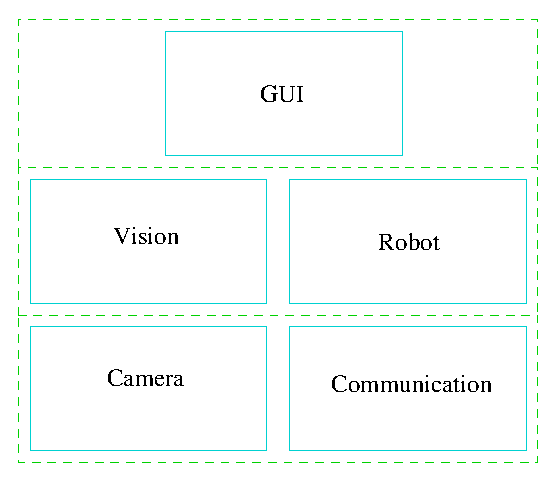
\includegraphics[width=8cm]{software-module}
  \caption{系统软件模块设计}
  \label{fig:software-module}
\end{figure}
Camera模块主要实现对偶RGB-D图像的匹配与合成,旨在提供高质量的RGB-D图像;Communication模块主要实现一个TCP服务器,并且定义了与机器人的通信协议,旨在提供与机器人高效稳定的通讯服务;Vision模块主要实现了3D-MRAI算法,旨在根据输入的RGB-D图像,输出目标工件的位姿;Robot模块主要实现与机器人相关的一些路径规划,根据目标工件的位姿生成机械臂抓取的位姿;GUI模块主要实现对检测结果的可视化,以及一些简单的流程控制。

所采用的嵌入式计算机使用的是嵌入式Linux操作系统,考虑到系统的性能以及算法的复杂性,整个系统软件使用C++编写。
\section{随机分拣实验}

\section{本章小结}

%%% Local Variables:
%%% TeX-master: "../thesis.tex"
%%% End: